\chapter[Przegląd istniejących rozwiązań][Przegląd istniejących
rozwiązań]{Przegląd istniejących rozwiązań}
Obecnie na rynku istnieje wiele dostępnych rozproszonych systemów plików,
zarówno komercyjnych, jak~i~darmowych. Swoje implementacje takich systemów
oferuje większość znaczących firm informatycznych, takich jak~Microsoft,
Google, Apache, Oracle, IBM czy RedHat. Poniżej zaprezentowane zostały dwa
wybrane rozproszone systemy plików.

\section[Google File System (GFS)][Google File System (GFS)]{Google File System
(GFS)}
GFS został zaprojektowany na~wewnętrzne potrzeby firmy Google, aby~przechowywać
duże ilości danych związanych z~pracą wyszukiwarki internetowej. W~systemie
wyróżnić można dwa rodzaje serwerów: Master oraz Chunkserver. Zadaniem tych
drugich jest przechowywanie wszystkich plików w~systemie. Pliki są~gromadzone
w~blokach (ang.~\emph{chunk}), każdy o~wielkości 64 megabajtów, które
replikowane są~pomiędzy kilkoma Chunkserverami (minimum trzy). Podczas operacji
czytania lub~przesyłania plików klient komunikuje się~bezpośrednio z~tymi serwerami.

\vspace{5mm}
Serwer Master jest z~kolei odpowiedzialny za~trzymanie wszystkich metadanych
o~plikach, czyli takich informacji jak odwzorowanie 64-bitowych etykiet plików
na~ich~lokalizację na~Chunk Serverach, lokalizację kopii bloków danych oraz
informacje o aktualnych operacjach wejścia i wyjścia w systemie. Wszystkie
te~dane są~aktualizowane poprzez periodycznie wysyłane komunikaty od~każdego z~serwerów.

\vspace{5mm}
Poniżej znajduje się schemat rozwiązania GFS:

\begin{figure}[H]
\center
\flushleft
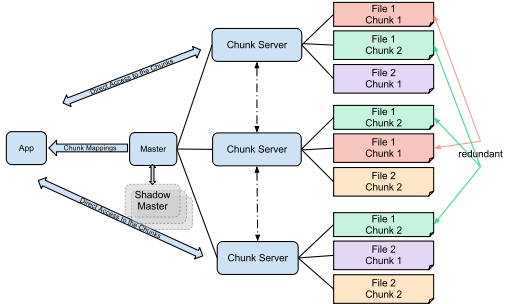
\includegraphics[keepaspectratio=true, scale=0.9]{img/gfs.png}
\caption{Źródło: http://en.wikipedia.org/wiki/Google\_File\_System}
\label{fig:gfs}
\end{figure}

\section[Hadoop File System (HDFS)][Hadoop File System (HDFS)]{Hadoop File
System (HDFS)}
Głównymi cechami, które wyróżniają ten rozproszony system plików od~innych jest
wysoka odporność na~błędy oraz skuteczność działania na~mniej wydajnym
sprzęcie. System ten~wchodzi w~skład rozwiązania open-source zwanego Apache Hadoop.

\vspace{5mm}
Podobnie jak~GFS, Hadoop File System składa się~z~głównego serwera zwanego
Namenode, który odpowiada za~usługi nazewnicze i~lokalizacyjne plików oraz
udostępnia interfejs dla~klienta. Dane są~przechowywane na~serwerach zwanych
Datanodes. Są~również pomiędzy nimi replikowane. Pliki mogą być przechowywane
w~całości lub~we~fragmentach.

\vspace{5mm}
Poniżej przedstawiony został schemat architektury HDFS:

\begin{figure}[H]
\center
\flushleft
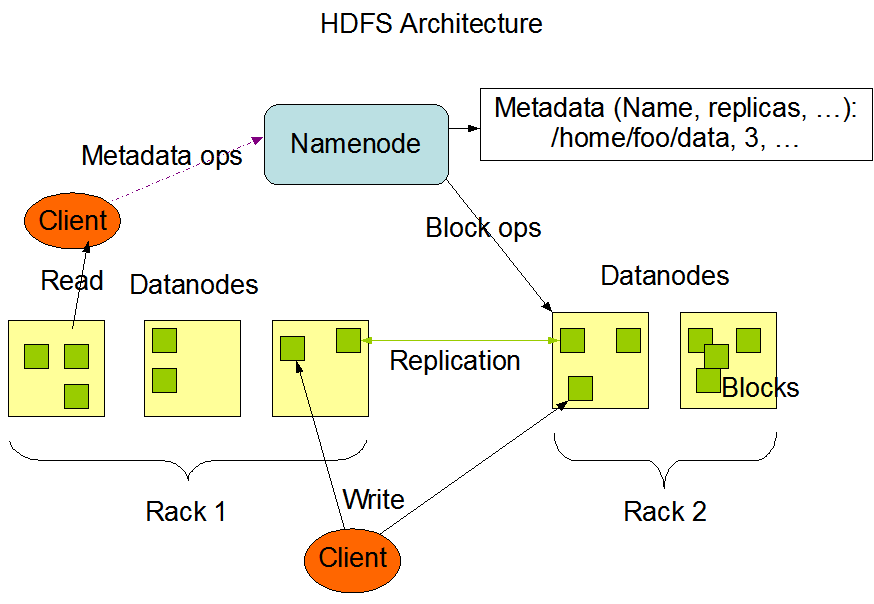
\includegraphics[keepaspectratio=true, scale=0.45]{img/hdfs.png}
\caption{Źródło: http://hadoop.apache.org/docs/r1.2.1/hdfs\_design.html}
\label{fig:hdfs}
\end{figure}

Lista innych przykładowych rozproszonych systemów plików:
\begin{itemize}
  \item Ceph (Inktank),
  \item FhGFS (Fraunhofer),
  \item GlusterFS (RedHat),
  \item Lustre,
  \item Windows Distributed File System (Microsoft).
\end{itemize}

\vspace{5mm}
Na przykładzie GFS oraz HDFS można zauwazyć, że~ogólny zamysł architektoniczny
rozproszonych systemów plików jest dość podobny. Większym różnicom podlegają
szczególy implementacyjne.
